\documentclass[a4paper,12pt,openany]{book}
\usepackage[T1]{fontenc}
\usepackage[utf8]{inputenc}
\usepackage{lmodern}
\usepackage{hyperref}
\usepackage{graphicx}
\usepackage{amsmath}
\graphicspath{ {images/} }
\usepackage[english]{babel}

%%%%%%%%%%%%%%%%%%%%%%%%%%%%%%%%%%%%%%%%%%%%%%%%
% Chapter quote at the start of chapter        %
% Source: http://tex.stackexchange.com/a/53380 %
%%%%%%%%%%%%%%%%%%%%%%%%%%%%%%%%%%%%%%%%%%%%%%%%
\makeatletter
\renewcommand{\@chapapp}{}% Not necessary...
\newenvironment{chapquote}[2][2em]
  {\setlength{\@tempdima}{#1}%
   \def\chapquote@author{#2}%
   \parshape 1 \@tempdima \dimexpr\textwidth-2\@tempdima\relax%
   \itshape}
  {\par\normalfont\hfill--\ \chapquote@author\hspace*{\@tempdima}\par\bigskip}
\makeatother

%%%%%%%%%%%%%%%%%%%%%%%%%%%%%%%%%%%%%%%%%%%%%%%%%%%
% First page of book which contains 'stuff' like: %
%  - Book title, subtitle                         %
%  - Book author name                             %
%%%%%%%%%%%%%%%%%%%%%%%%%%%%%%%%%%%%%%%%%%%%%%%%%%%

% Book's title and subtitle
\title{\Huge \textbf{EVM Design}}\\ 
% Author
\author{\textsc{Deepanshu Jindal}}\\

\begin{document}

\frontmatter
\maketitle

\tableofcontents

\mainmatter

%%%%%%%%%%%
% Preface %
%%%%%%%%%%%
\chapter*{Preface}
This is a document which details the features of an ideal EVM and discusses the problems with the current EVM design in the country. Finally it looks upon a possible design of EVM which attempts to meet the features detailed in the first section.
\\


\chapter{What we expect from EVM}

\section{Coercion freedom}
We want the EVM to protect the voter's Right to Choice. We wish to ensure that the voter cannot be coerced by anybody to change his voting choice in an unfair way.
\\
This is closely tied to secrecy of vote as coercion freedom also means that nobody can determine with certainty to whom the voter voted by use of coercion.

\section{Secrecy}
Secrecy that if the voter doesn't want to disclose to whom he/she voted, then it should not be possible for anyone to determine with certainty that who the voter voted for.

\section{Anonymity}
The identity of the voter should be protected in all circumstances. Nobody should be able to identify a voter from the data of voting.

\section{Non-repudiation}
Nonrepudiation is the assurance that someone cannot deny something. Typically, nonrepudiation refers to the ability to ensure that a party to a contract or a communication cannot deny the authenticity of their signature on a document or the sending of a message that they originated. 
\\
In the context of voting it means that a voter cannot challenge that his vote was registered for a party different from whom he/she voted for.

\section{Verifiability}
Voter should be able to verify that his/her vote is counted towards the party he/she has voted for.\\
It should be possible to easily verify that the EVM is not tampered with. The authenticity of both hardware and the software of the EVM should be provable.

\section{Cryptosecure}
The data stored in EVM should be encrypted and cryptographically secure, so that any unauthorised third party cannot access it or tamper with it.

\section{Auditable}
It should be provable that the EVM works without any bias. There should be a proof of correctness of the entire process of voting. It should be possible to audit the process of voting at any stage and detect discrepancies if any.

\section{Self-certifiability}
The hardware and software should be self certifiable and tamper detection should be possible if one of them is compromised.

\section{Protection from information leakage}
The data stored inside the EVM should be protected from any kind of leakages. No third party should be able to access any sort of data from EVM during the process of voting and counting.

\section{Constraints under which EVM are required to work}


\begin{itemize}
\item Cost effectiveness
\item Lack of electricity in remote areas
\item Illiteracy and unfamiliarity towards technology amongst population enforces adoption of simplistic designs
\item Booth capture
\end{itemize}

\chapter{The current design}
Elections in India are conducted almost exclusively using electronic voting machines developed over
the past two decades by a pair of government-owned companies. These devices, known in India as EVMs,
have been praised for their simple design, ease of use, and reliability, but recently they have also been
criticized following widespread reports of election irregularities.

\section{Operations and Procedure}
\begin{figure}[!h]
\centering
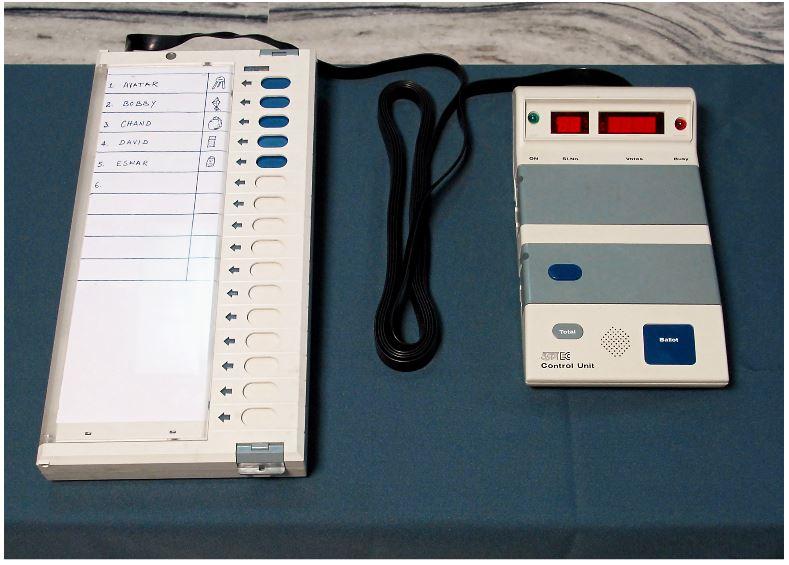
\includegraphics[scale=0.4]{EVM_with_Control_Unit.JPG}
\caption{The ballot and the control unit of EVM}
\end{figure}
\\
EVM consisted of two main components : Ballot unit and Control Unit.
Control Unit is used by poll
workers, which stores and accumulates votes.
Ballot Unit
is located in the election booth, which is
used by voters. These units are connected by a 5 m cable, which has one end permanently fixed to the ballot
unit.


The ballot unit has 16 candidate buttons. If any are unused, they are covered with a plastic masking tab
inside the unit. When there are more than 16 candidates, an additional ballot unit can be connected to a port on
the underside of the first ballot unit. Up to four ballot units can be chained together in this way, for a maximum
of 64 candidates.\\

Recently, a new unit called VVPAT was added to EVM to improve verifiability. Voter Verifiable Paper Audit Trail (VVPAT) or Verifiable Paper Record (VPR) is a method of providing feedback to voters using a ballotless voting system. A VVPAT is intended as an independent verification system for voting machines designed to allow voters to verify that their vote was cast correctly, to detect possible election fraud or malfunction, and to provide a means to audit the stored electronic results.

\section{Issues with the design}
lack of encryption

\begin{thebibliography}{9}
\bibitem{2Dto3D}
Security Analysis of India’s Electronic Voting Machines
\url{https://indiaevm.org/evm_tr2010-jul29.pdf}

\bibitem{VVPAT}
Voter-verified paper audit trail
\url{https://en.wikipedia.org/wiki/Voter-verified_paper_audit_trail}


\end{document}
